\documentclass{beamer}

\mode<presentation>
{
\usetheme{Dresden} 
%\usecolortheme{spruce}
\usefonttheme{professionalfonts}
%\setbeamercovered{invisible}
%\setbeamertemplate{itemize subitem}[triangle]
\setbeamertemplate{blocks}[rounded]
\setbeamertemplate{footline}
{
  \leavevmode%
  \hbox{%
  \begin{beamercolorbox}[wd=.25\paperwidth,ht=2.25ex,dp=1ex,left]{title in head/foot}%
    \usebeamerfont{author in head/foot}\hspace*{2ex}\insertauthor
  \end{beamercolorbox}%
  \begin{beamercolorbox}[wd=.5\paperwidth,ht=2.25ex,dp=1ex,center]{date in head/foot}%
    \usebeamerfont{title in head/foot}\inserttitle
  \end{beamercolorbox}%
  \begin{beamercolorbox}[wd=.175\paperwidth,ht=2.25ex,dp=1ex,right]{title in head/foot}%
    \usebeamerfont{date in head/foot}\insertshortdate{} \hspace*{2ex}
  \end{beamercolorbox}}%
  \begin{beamercolorbox}[wd=.075\paperwidth,ht=2.25ex,dp=1ex,center]{date in head/foot}%
    \insertframenumber{} / \inserttotalframenumber
  \end{beamercolorbox}%
  \vskip0pt%
}
}

\usepackage{amsmath}
\usepackage{amsfonts}
\usepackage{graphicx}
\usepackage[english]{babel}
\usepackage[utf8]{inputenc}
\usepackage[T1]{fontenc}
\usepackage{multirow}
\usepackage{rotating}
\usepackage[scaled=.90]{helvet}
\usepackage{xcolor}
\usepackage[T1]{fontenc}
\usepackage{abbrevs}


\beamertemplatenavigationsymbolsempty
\setbeamerfont{footnote}{size=\tiny}
\setbeamertemplate{itemize subitem}[triangle]


\title{A critical review of age-related research on L2 ultimate attainment}
\author{A. Wachtler and C. Jenkins}
\institute{Institut f\"ur Maschinelle Sprachverarbeitung, Universit\"at Stuttgart\\Probabilistic Graphical Models for Natural Language Processing}
\date{6 July 2016}

\begin{document}

\AtBeginSection[]{
  \begin{frame}
  \vfill
  \centering
  \begin{beamercolorbox}[sep=8pt,center,shadow=true,rounded=true]{title}
    \usebeamerfont{title}\insertsectionhead\par%
  \end{beamercolorbox}
  \vfill
  \end{frame}
}


% Cover Page
\begin{frame}
  \titlepage
\end{frame}

% Outline
 \begin{frame}{Outline}
   \tableofcontents
 \end{frame}

\begin{frame}{Recap - last week}
    % dealing with difficulties in studying SLA
    % use of a computational model to create a well-defined, controlled situation
    The Bilingual Language Interaction Network for Comprehension of Speech.
    \begin{itemize}
      \item Problem: 2nd Language acquisition has many factors
      \item These are difficult to control for in experimental groups 
      \\
      \item Approach: computational model of bilingualism
      \begin{itemize}
        \item BLINCS model
        \item Operates at semantic, phonological, lexical, orthographic levels
        \item Incorporates L1 knowledge
      \end{itemize}
    \end{itemize}
\end{frame}

\begin{frame}{This week's paper}
    \begin{center}
        A critical review of age-related research on L2 ultimate attainment \\
        By Carmen Muñoz and David Singleton \\
        Appeared in Language Teaching vol. 44
    \end{center}
\end{frame}

\section{Overview}

\begin{frame}{Prelude to a Contentious Topic}
  \begin{itemize}
    \item The authors offer some good advice:
    \begin{itemize}
      \item Respect your colleagues
      \item Even if you diasgree with their approach
      \item Science is a laborious process
    \end{itemize}
  \end{itemize}
  
\end{frame}

\section{L1-Speaker Benchmark}

\section{Definition(s) of Crit. Period}

\begin{frame}{Conflicting Definitions}
  Different critical points for various components of language
  \begin{itemize}
    \item Phonology

    \item Syntax

    \item Lexicon
  \end{itemize}
\end{frame}

\begin{frame}{Other Critical Periods}
  \begin{itemize}
    \item Bionocular vision
    \begin{itemize}
      \item Input from both eyes needed at a young age
    \end{itemize}
    \item Imprinting
    \begin{itemize}
      \item Some bird species quickly learn to follow someone
      \item Ideally this is their parent
    \end{itemize}
    \item Ethical concerns
  \end{itemize}
\end{frame}

\begin{frame}{Dramatic Dropoff}
  \begin{itemize}
    \item ``Elbow shape'' dropoff?
    \begin{itemize}
      \item Severe difference in language learning ability
      \item \emph{Qualitative} difference
    \end{itemize}
    \item Gradual decline
    \begin{itemize}
      \item Age-related cognitive deterioration
      \item \emph{Linear} decline throughout life
    \end{itemize}
  \end{itemize}
\end{frame}

\begin{frame}{Comparing Studies} % overall fuzziness
\end{frame}

\section{Contextual Factors}

\begin{frame}{Classic Benchmarks} % discussing Age of Acquisition, Length of Residence, pros, cons
    \begin{itemize}
        \onslide<2->\item Age of Acquisition (AoA)
        \onslide<3->\item Length of Residence (LoR) \\
       \onslide<4->\item Positive:
        \begin{itemize}
          \onslide<5->\item Easy to obtain
        \end{itemize}
       \onslide<6->\item Negative:
        \begin{itemize}
         \onslide<7->\item Much variation not accounted for
        \end{itemize}
        % moving beyond these
    \end{itemize}
\end{frame}

\begin{frame}{Social Factors} % this could really be several slides
  \begin{itemize}
    \item Exposure to language input can be limited by circumstances
    \begin{itemize}
      \item Even in a country where that language is predominantly spoken
    \end{itemize}
  \end{itemize}
  \onslide<2->\begin{columns}
    \column{0.5\textwidth}
      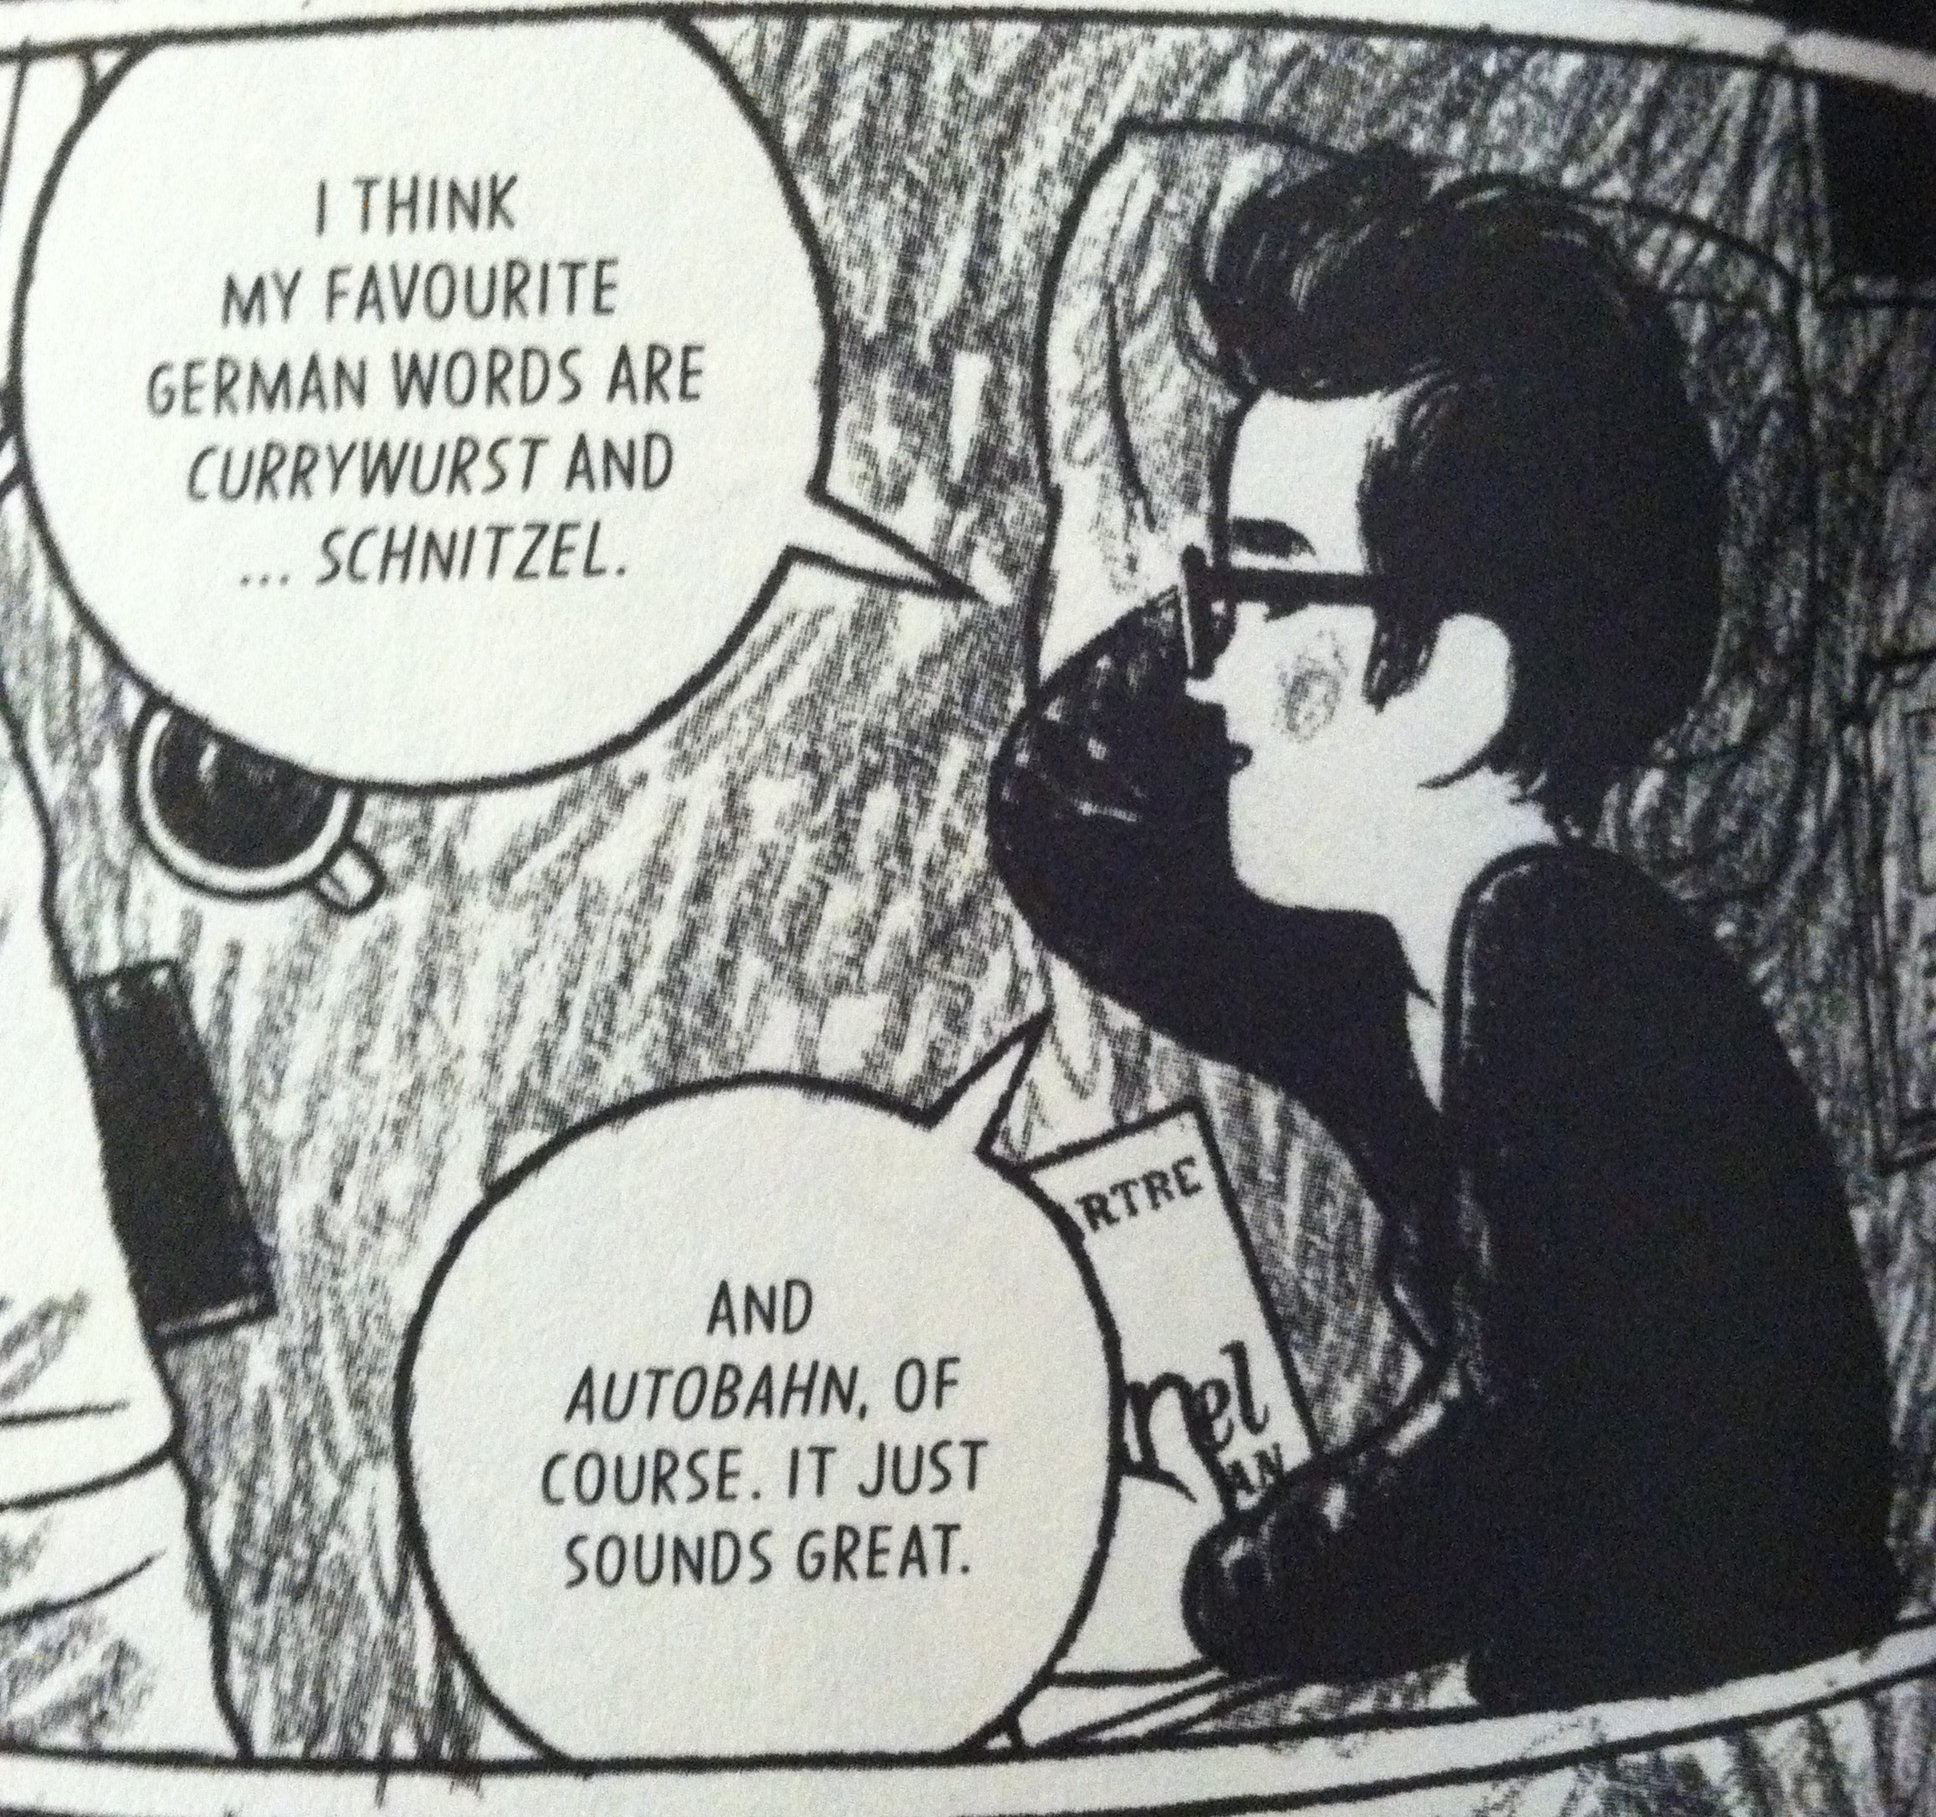
\includegraphics[scale=0.07]{currywurst_cropped.JPG} \\
      \tiny{\textit{Baby's in Black} by Arne Bellstorf}
    \column{0.5\textwidth}
      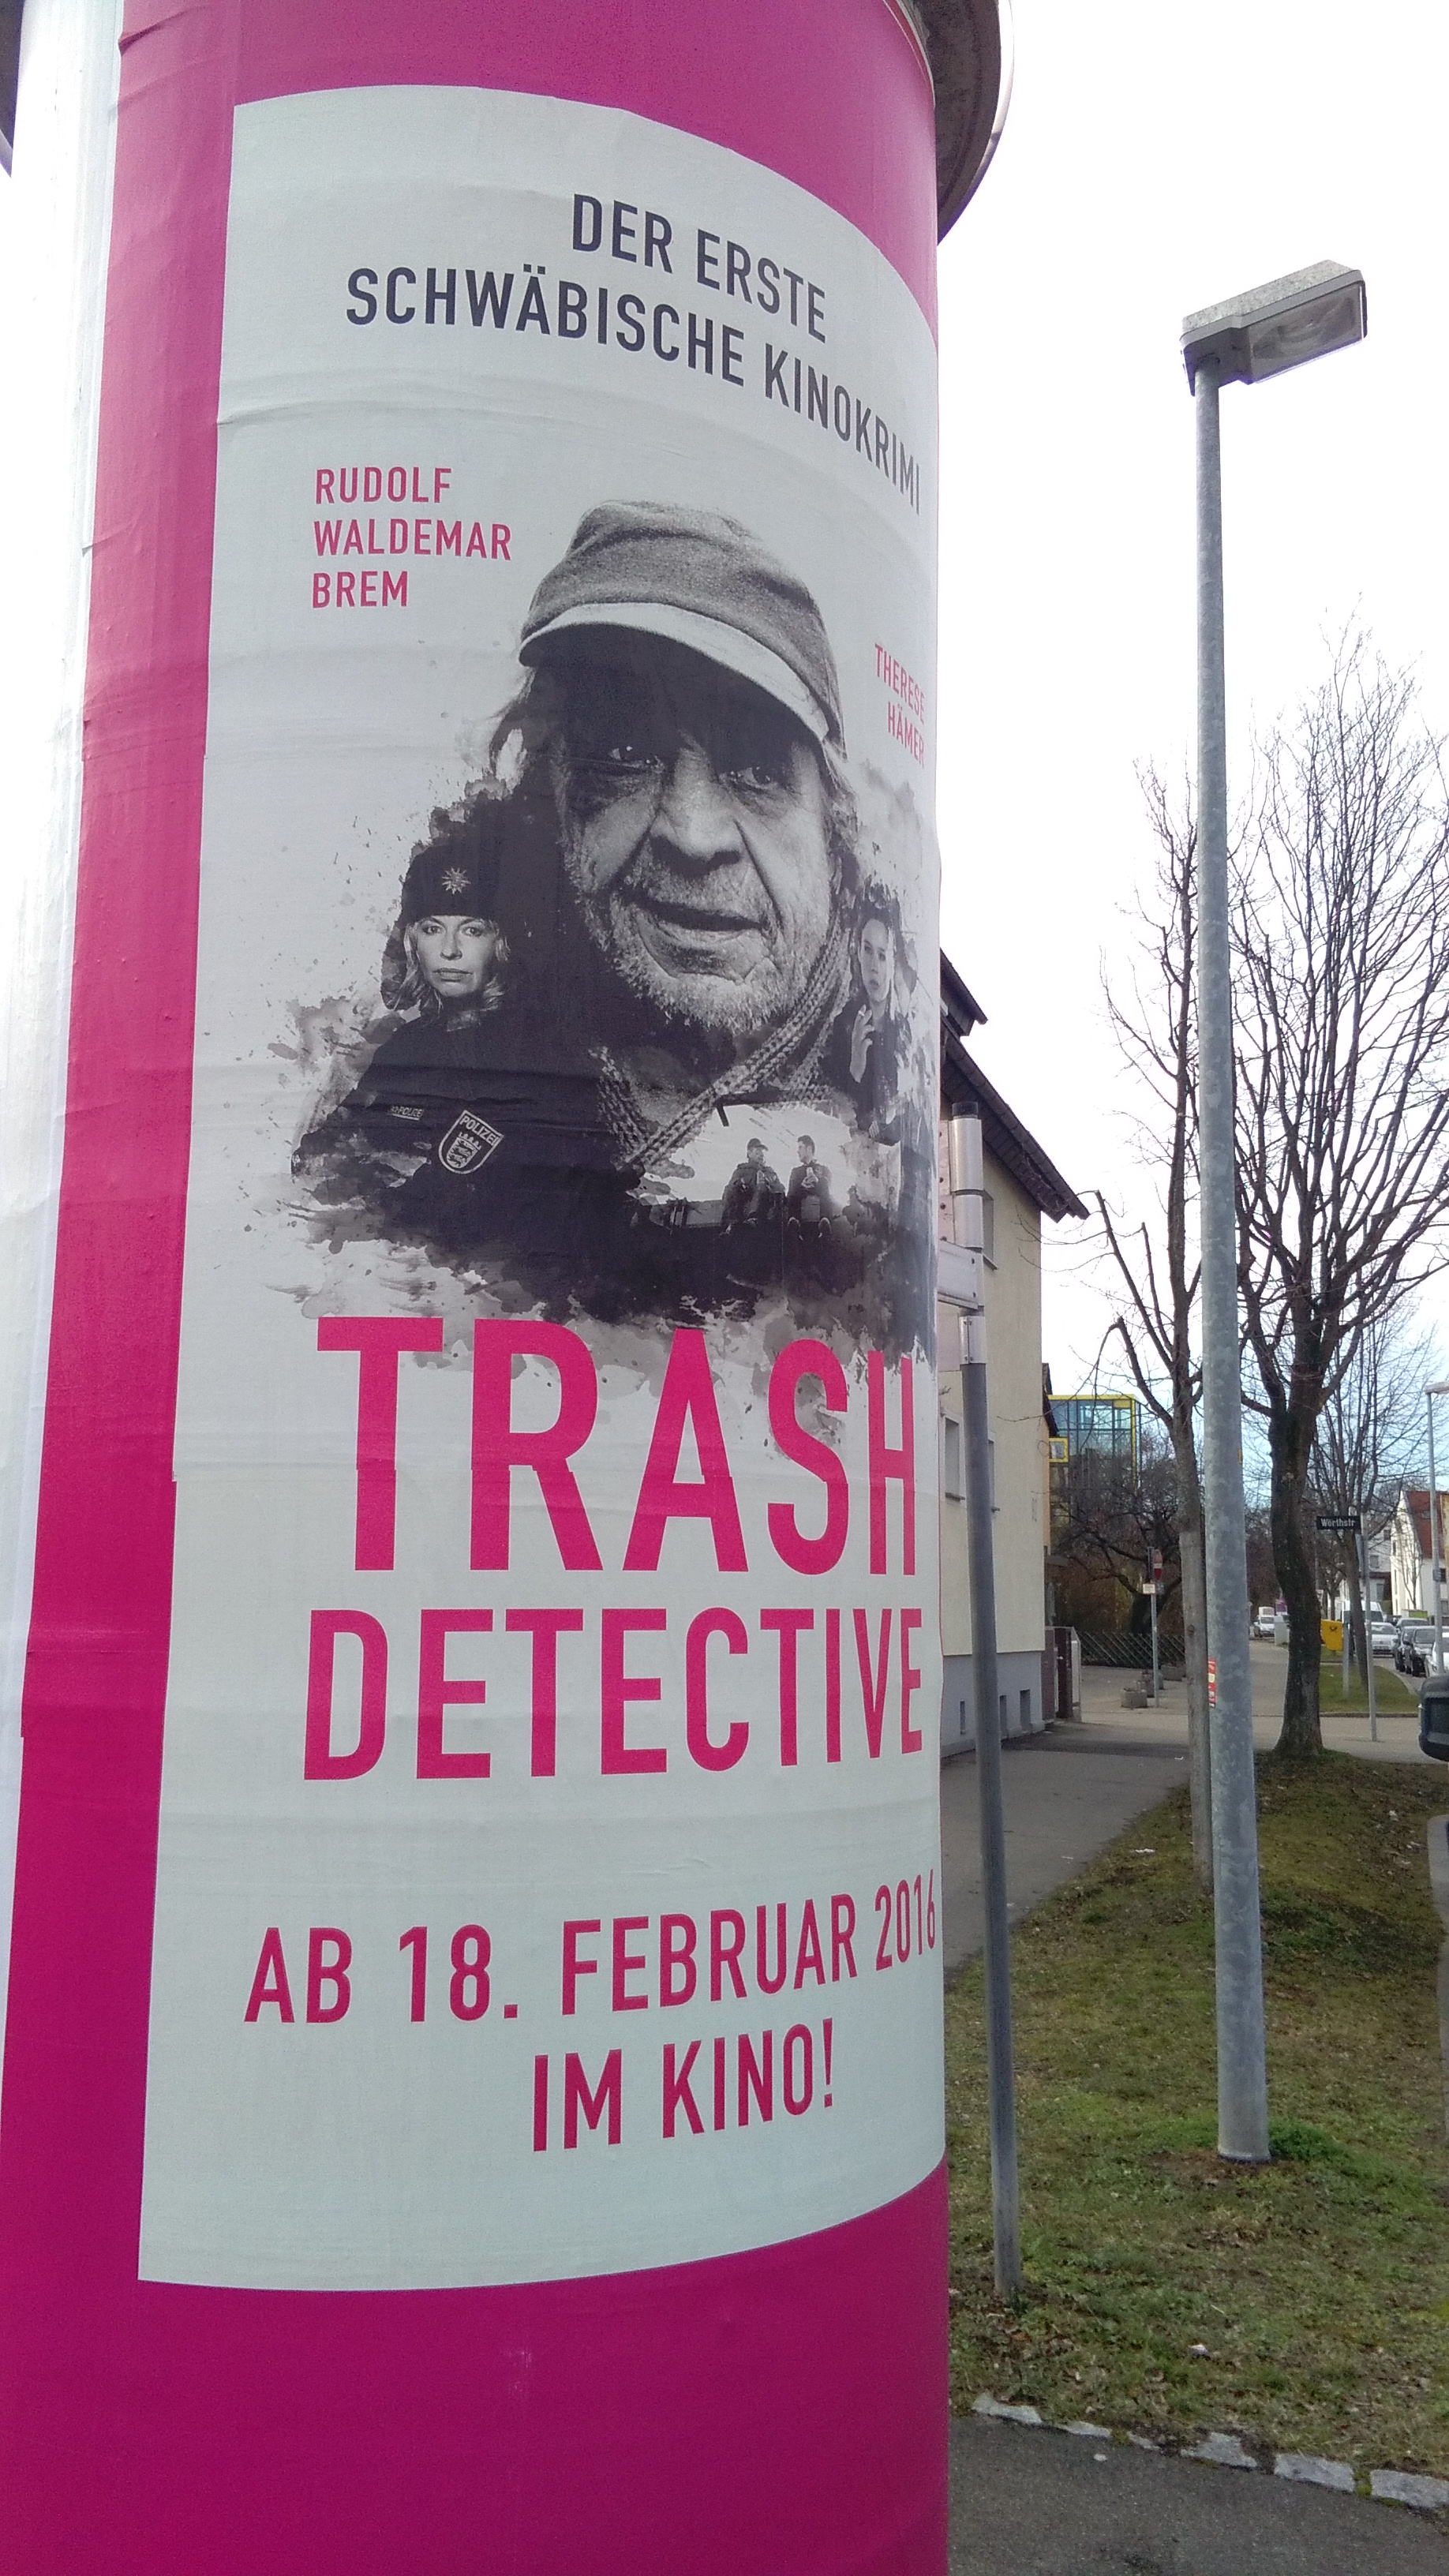
\includegraphics[scale=0.05]{trash_detective.jpg}
  \end{columns}
\end{frame}

\begin{frame}{Social Factors}
  \begin{itemize}
    \item Social factors can affect \emph{exposure} to and \emph{use} of L2
  \end{itemize}
\end{frame}

\begin{frame}{Identity}
  
\end{frame}

\begin{frame}{Feedback Loop}
  \begin{itemize}
    \item Language experience builds on experience
    \begin{itemize}
      \item More opportunities to have conversations
    \end{itemize}
    \item Earlier L2 learning could correspond to family, friend, community groups
    \item Confidence, sense of self
  \end{itemize}
\end{frame}

\begin{frame}{Study Methodology}
    \begin{itemize}
        \item Interview Questions
        \item Longitudinal Studies
    \end{itemize}
\end{frame}

\section{Neurolinguistic Considerations}

\section{Takeaway}

\end{document}